% =====================================================================
% The Central Dark Mass of Omega Centauri: A Pre-registered Joint
% Analysis and Why the Data Cannot Yet Decide  (Paper H)
% Tim Swanson — The Omega Centauri Society / Post Oak Labs
% Build: pdflatex mass-tension-paper && bibtex mass-tension-paper
%        && pdflatex x2
% Machinery + results: paper/h/ (data, mock, jerk, g3, fit, fit2);
% pre-registration incl. amendments A1/A2: paper/H-PREREGISTRATION.md;
% referee record: OCS-REFEREE-H-FIT-REVIEW_2026-08-13.md.
% =====================================================================
\documentclass[11pt]{article}

\usepackage[margin=1.1in]{geometry}
\usepackage{newtxtext,newtxmath}
\usepackage[round,authoryear]{natbib}
\usepackage{graphicx}
\usepackage{booktabs}
\usepackage{amsmath}
\usepackage{tikz}
\usepackage{pgfplots}
\pgfplotsset{compat=1.17}
\usepgfplotslibrary{fillbetween}
\usepackage[font=small,labelfont=bf]{caption}
\usepackage{microtype}
\usepackage[colorlinks=true,linkcolor=blue!50!black,citecolor=blue!50!black,urlcolor=blue!50!black]{hyperref}
\usepackage{xcolor}

\newcommand{\msun}{\ensuremath{M_\odot}}
\newcommand{\ocen}{$\omega$~Cen}
\newcommand{\mdark}{\ensuremath{M_{\mathrm{dark}}}}
\newcommand{\lnK}{\ensuremath{\ln K}}
\newcommand{\kms}{\ensuremath{\mathrm{km\,s^{-1}}}}
\newcommand{\specbox}[1]{\par\smallskip\noindent\fbox{\parbox{0.97\linewidth}{\small\textbf{Epistemic status:} #1}}\smallskip\par}

\title{\textbf{The Contested Central Dark Mass of Omega Centauri:\\ A Pre-registered Joint Analysis of Fast Stars, Pulsar Timing,\\ and the Limits of the Proper-Motion Dispersion Profile}}
\author{Tim Swanson\\[2pt]
\small The Omega Centauri Society / Post Oak Labs\\
\small \texttt{tim@postoaklabs.com}}
\date{August 2026 \\[4pt] \small Draft v0.3 (last revised 2026-08-14) --- seventh paper of the set (Paper H); companion to the Macro Transcension\\ \small Hypothesis (Paper A), the inward-migration review (Paper B), the Omega Centauri campaign (Paper C), the migration\\ \small economics (Paper D), the engineered-IMBH systems paper (Paper E), and the joint accretion bound (Paper F);\\ \small prepared for omegacentauri.me}

\begin{document}
\maketitle

\begin{abstract}
\noindent
The center of Omega Centauri carries the sharpest unresolved mass question in globular-cluster dynamics: seven fast-moving stars inside the central $3''$ imply an enclosed dark mass $\gtrsim 8{,}200\,\msun$ \citep{Haberle2024Nature}, while joint stellar-kinematics and pulsar-timing modeling favors an extended $\sim 2$--$3\times10^{5}\,\msun$ remnant component and caps any point mass at $\lesssim 6{,}000\,\msun$ \citep{BanaresHernandez2025}. We report the first joint likelihood analysis of the individual fast stars, the 19-pulsar TRAPUM timing set \citep{ColomiBernadich2026} read correctly as one-sided acceleration bounds, and the oMEGACat 40-bin proper-motion dispersion and anisotropy profiles \citep{oMEGACatVI2025}, with the dark component parameterized continuously in mass and scale radius from the point-mass limit to the extended-cluster regime. The analysis was pre-registered before real-data contact, with prior grids, decision criteria, and validation gates fixed in advance and two dated amendments disclosed. The pre-registered outcome is the one we report: the data cannot yet decide between a compact and an extended central dark mass, and we can now say why, quantitatively, for each data type. The dispersion profile, measured to 0.03--0.05\,\kms, rejects every smooth spherical non-rotating model ($\chi^{2}/\nu \approx 473$ in the outer bins) through a coherent, component-differential residual that no radial systematic term can absorb; its verdict-dominant bins lie at radii carrying under $10^{-3}$ of the dark component's enclosed-mass signal, so the leg's formal power is spurious precision, and we retire it from the verdict by a pre-set gate. The pulsar accelerations, all censored, span 3.0 nats across the entire parameter plane. The pulsar spin-frequency second derivatives are inconsistent with cluster jerks and, after correcting a numerical constant in the published nearest-neighbour jerk scale ($\xi = 3.4596$, not 3.04), we show jerk discrimination requires a timed-pulsar census of order $10^{2}$, several times the 19 available, at any timing precision, because the nearest-neighbour floor is a 1-stable process that does not average away. The fast-star leg alone, under the assumed tracer cusp, returns a compact optimum ($\mdark \approx 2.0$--$2.5\times10^{4}\,\msun$ at the point-mass limit, $\lnK = +10$ to $+12$; range over all prior cells and brackets, Section~\ref{sec:record}), which we report and do not promote: the injection-calibration gate shows the machinery under-covers on the extended alternative, and a preference certified by an uncalibrated instrument is not a measurement. A formation-physics overlay sharpens the impasse from the other side: published retention physics builds the compact solution readily and reaches the extended solution only through hybrid configurations that the extended solution's own point-mass cap excludes. We state what would decide the question, and in which order.
\end{abstract}

\bigskip
\noindent\textbf{Keywords:} globular clusters: individual (NGC 5139); intermediate-mass black holes; stellar dynamics; pulsars: timing; methods: statistical; pre-registration

\newpage
\tableofcontents
\newpage

\section{Introduction}
\label{sec:intro}

\ocen{} (NGC 5139) has hosted claims and counter-claims of a central intermediate-mass black hole (IMBH) for nearly two decades: integrated-light kinematics for $\sim 4\times10^{4}\,\msun$ \citep{Noyola2008,Noyola2010H}, proper-motion modeling capping the mass at $\lesssim 1.2\times10^{4}\,\msun$ with the verdict hinging on the adopted center \citep{vanderMarelAnderson2010}, radial anisotropy shown to mimic much of the signal \citep{Zocchi2017}, stellar-mass black-hole populations shown to mimic more of it \citep{Zocchi2018,Baumgardt2019}. The modern form of the question is sharper on both sides. \citet{Haberle2024Nature} found seven fast-moving stars inside the central $3''$, five robust, with velocities above the central escape speed of any IMBH-free model, giving a firm kinematic lower bound of $8{,}200\,\msun$ on an enclosed dark mass. \citet{BanaresHernandez2025} combined stellar kinematics with millisecond-pulsar accelerations and found the data favor an extended dark component of $2$--$3\times10^{5}\,\msun$ at parsec scale, with a $3\sigma$ cap of $6{,}000\,\msun$ on any point mass, below the fast-star bound. The TRAPUM timing release \citep{ColomiBernadich2026} expanded the pulsar census to 19 with an IMBH-insensitive upper limit of $10^{5}\,\msun$, sharpening the data without resolving the contradiction.

The methodological history of this exact contest in other clusters is cautionary in both directions. In 47 Tucanae, a pulsar-dynamics IMBH claim \citep{Kiziltan2017} did not survive multimass remnant modeling \citep{Mann2019,Smith2024}; in NGC 6397, a claimed IMBH resolved into a diffuse inner subcluster \citep{VitralMamon2021}; and \citet{Aros2020} showed with mock data that Jeans-type fits fabricate IMBH masses at this scale when anisotropy or mass-to-light structure is mis-modeled. Any new joint analysis of \ocen{} enters a literature where the last three comparable verdicts were overturned by systematics, and it should be built accordingly.

This paper reports such an analysis, built with three defenses the prior literature lacked in combination. First, a genuinely joint likelihood: the individual fast stars (velocities, positions, selection function, contamination), the pulsar line-of-sight accelerations read as the one-sided bounds they are, and the dispersion and anisotropy profiles, all constraining one dark component parameterized continuously by mass \mdark{} and Plummer scale $a$, from the point-mass limit ($a \to 0$) to the extended-cluster regime, so that the compact and extended hypotheses are regions of one parameter plane rather than separate models with separate machinery. Second, pre-registration: the prior grid, the decision criteria, the validation gates, and the amendment protocol were committed to a public repository before any likelihood touched real data, and both subsequent amendments are dated and disclosed (Section~\ref{sec:prereg}). Third, adversarial validation: the pipeline had to reproduce the \citet{Aros2020} failure mode on demand (inject anisotropy, fit isotropic, measure the fabricated mass) and demonstrate calibrated coverage on mock injections before first real-data contact, and a second gate battery governed what became quotable afterward.

The outcome is the pre-registered null: the data cannot yet decide. We consider that outcome, reached this way, more useful than another overturnable verdict, because the machinery now localizes the indecision to specific, named causes per data type, and because the same machinery yields the first quantitative statement of what a deciding dataset must contain. Sections~\ref{sec:data}--\ref{sec:machinery} describe the data, the pre-registered design, and the validated machinery, including a correction to a published constant in the pulsar-jerk formalism that other groups may wish to note independently of anything else in this paper. Sections~\ref{sec:fit}--\ref{sec:diagnosis} report the joint fits under both pre-registered error models and diagnose, leg by leg, where the discriminating power actually resides. Section~\ref{sec:formation} adds the formation-physics overlay, Section~\ref{sec:decide} states what would decide the question, and Section~\ref{sec:conclusion} concludes.

\section{Data}
\label{sec:data}

All inputs were extracted from their primary sources into versioned, provenance-annotated tables before any modeling, with every value carrying its source location and verbatim context; the fit records the content hash of each input it consumed. Four datasets enter.

\textbf{Fast stars.} The seven candidates of \citet{Haberle2024Nature}, with the robust/candidate split preserved: the headline analysis uses the five robust stars (A, C, D, E, F), and the all-seven variant is a reported sensitivity row. Positions, proper motions, and uncertainties come from their Extended Data tables; the selection function is reconstructed from the stated quality-cut pass fraction (157{,}320 of 241{,}133 stars, completeness 0.652), the $3''$ search radius, the 2.41\,mas\,yr$^{-1}$ threshold, and the published contamination density, which reproduces the paper's own expected foreground count (0.0735 against their quoted 0.074). The N-body-informed mass range quoted in that paper's methods is model output, not data, and enters nowhere in this analysis.

\textbf{Pulsar accelerations.} The TRAPUM timing solutions \citep{ColomiBernadich2026}: 8 of 19 pulsars have measured spin-period derivatives; every derived cluster line-of-sight acceleration is a one-sided bound, because the intrinsic spin-down is unknown and non-negative. Seven bounds enter the likelihood; one (pulsar C) is excluded because its published table entry is typeset in a form we could not disambiguate, and we do not silently repair source tables. Three of the seven bounds are negative-signed (B, D, K), and those carry what constraining power the leg has. We verified the published reduction chain by recomputing pulsar A's bound from its $P$, $\dot{P}$, and the Shklovskii and Galactic terms ($1.9796\times10^{-9}$ against the printed $1.98\times10^{-9}$\,m\,s$^{-2}$). The earlier five-pulsar solutions of \citet{Dai2023} are carried as a labelled sensitivity variant; Section~\ref{sec:diagnosis} reports what that comparison revealed.

\textbf{Dispersion, anisotropy, rotation.} The oMEGACat 40-bin sky-radial and sky-tangential proper-motion dispersion profiles with their anisotropy ratios, $r = 1.8''$--$311''$, statistical errors 0.023--0.05\,\kms{} in the best-measured bins, retrieved from the survey's machine-readable release and checksum-verified \citep{oMEGACatVI2025}; the integrated-light rotation profile (amplitude rising to $8.4 \pm 0.8$\,\kms{} at $4.7'$) frozen from \citet{Haberle2026LVM}; kinematic distance $5{,}494 \pm 61$\,pc from the same survey, with the 5{,}200\,pc value adopted by \citet{BanaresHernandez2025} carried as a reported axis rather than harmonized away.

\textbf{Visible-model structure.} No machine-readable radial surface-brightness array for \ocen{} exists in the public record; we verified this against the survey chain, the \citet{BaumgardtHilker2018} catalogue release, and its archival files before concluding it, and the gap forced Amendment A1 below. The visible model is therefore the reported pair: a Plummer sphere at the catalogue half-light scale, and the published $\alpha\beta\gamma$ profile of \citet{BanaresHernandez2025} at its released best-fit parameters, each normalized on the outer dispersion bins ($r > 100''$), where the dark component contributes below one part in $10^{3}$ of the enclosed mass everywhere in the prior grid.

\section{Pre-registered design}
\label{sec:prereg}

\specbox{This section describes process, not results. The pre-registration file, its git history, both amendments, the referee reports that produced Amendment A2, and every validation and fit report are distributed with the paper source; each claim in this section is checkable against a committed document that predates the result it governs.}

The analysis plan was committed before any real-data likelihood evaluation. Its elements: (i) the model, one dark Plummer component with $(\mdark, a)$ continuous over $[10^{3}, 10^{6}]\,\msun \times [10^{-4}, 3]$\,pc, the point-mass limit included; (ii) prior-sensitivity sweeps over sub-ranges of both axes, with mass-function and retention nuisances bracketed rather than point-chosen; (iii) decision criteria fixed in advance, including the rule that any compact-versus-extended Bayes factor is reported only as a table over all prior cells, that no $|\lnK| < 1$ appears in the abstract, and that ``the data cannot decide'' is a declared, publishable outcome with a mechanical trigger (criterion 3 unmet in at least half the prior cells); (iv) validation gates that had to pass before real-data contact: injection--recovery with calibrated coverage including the \citet{Aros2020} anisotropy reproduction (G1), validation of the jerk-statistics module against the published analytic distributions (G2), and a formation-channel consistency map that never enters the likelihood (G3).

Two amendments were required, both dated, both disclosed here. \textbf{A1:} the pre-registered fiducial visible model was defined on a surface-brightness profile that turned out not to exist in machine-readable form; the amendment names the Plummer/$\alpha\beta\gamma$ pair as a reported bracket, neither member promoted. \textbf{A2:} the first real-data run exposed that the dispersion profile's assumed error model controlled the compact-versus-extended verdict outright (Section~\ref{sec:fit}); rather than choose a value, we froze the run and took the question to two independent methodological reviews and, on their split, a tiebreak adjudication, whose ruling was adopted verbatim: all quadrature error floors, fixed or fitted, were struck as primary (a coherent one-signed residual is mean-model bias, and inflating variance against a biased mean is equivalent to deleting the leg gradually), replaced by an explicit mean-model discrepancy term in the style of \citet{KennedyOHagan2001}, a four-knot spline in $\log r$ with physics-scaled priors and a small white term, both marginalized, together with four quotability gates: a sign and runs test on the residuals, sign-unanimity of \lnK{} across every prior cell and bracket, an injection-calibration rerun at real-data precision with deliberate coherent misspecification, and a budget-overrun kill switch that retires the leg from the verdict if the required discrepancy exceeds twice its physics budget.

The amendments changed the error model. They did not change the priors, the criteria, the data, or the quotability rules, and the second was adopted with its gates fixed before the rerun that they then failed. One further process deviation is disclosed here rather than discovered later: the first run derived its mass-to-light bracket from its own calibration statistics instead of the pre-registered retention-anchored brackets; the deviation was identified in review, folded into the A2 record, and the bracket re-derived under the amended error model (its half-width widening from 4 to 9.7\,per~cent, the honest direction).

\section{Machinery and validation}
\label{sec:machinery}

\subsection{Joint likelihood and gate G1}
\label{sec:g1}

The three legs share one potential: visible model plus dark Plummer component. The fast-star leg evaluates each star's proper-motion speed against the local high-velocity tail of a truncated-polytrope speed distribution matched to the Jeans solution, with the selection function, completeness, and contamination in the likelihood, and a Bahcall--Wolf tracer cusp \citep{BahcallWolf1976} applied identically in generation and fitting inside the dark component's influence radius. The pulsar leg computes the probability that the model line-of-sight acceleration lies below each one-sided bound, with the unknown line-of-sight positions marginalized over the tracer density in the manner of \citet{Prager2017}. The profile leg fits both dispersion components with radial anisotropy marginalized over an Osipkov--Merritt scale grid, never fixed isotropic.

Gate G1 required, on mocks: calibrated 90\,per~cent coverage for a $4\times10^{4}\,\msun$ point-mass injection and a $2.5\times10^{5}\,\msun$ extended injection (achieved: 0.84 and 0.92, inner quantiles under-covering, declared and flagged as approximate); no manufactured detection on a null injection (0.00); compact/extended false-preference rates below 0.10 (0.02 and 0.00); and the \citet{Aros2020} reproduction, which we regard as the gate's core: mocks generated with radial anisotropy and no dark mass, fitted with isotropy forced, manufacture $8.0\times10^{4}\,\msun$ of dark mass and a 76\,per~cent spurious detection rate; the same data under the pre-registered anisotropy marginalization return a null with a 0\,per~cent spurious rate. The degeneracy that overturned prior verdicts is reproducible on demand and demonstrably closed by the marginalization.

\subsection{The jerk module, gate G2, and a correction to a published constant}
\label{sec:jerk}

Pulsar spin-frequency second derivatives probe a central mass through the jerk field, against a stochastic floor from nearest-neighbour stellar encounters \citep{Prager2017,Abbate2019}. Implementing that formalism, we found the published value of the dimensionless constant in the nearest-neighbour jerk scale, $\dot{a}_{0} = (2\pi\xi/3)\,G\langle m \rangle \sigma n$, to be in error. The defining double integral evaluates in closed form:
\begin{equation}
\xi = \int_{0}^{\infty}\!\!\mathrm{d}x \int_{-1}^{1}\!\!\mathrm{d}\mu \left[ 1 - e^{-(1+3\mu^{2})/(2x^{2})} \right]
 = \sqrt{2\pi}\left[ 1 + \frac{\ln(2+\sqrt{3})}{2\sqrt{3}} \right] = 3.4596,
\end{equation}
against the published $\xi \simeq 3.04$, a 13.8\,per~cent difference confirmed by six independent routes (closed form, direct quadrature, a Poisson-field Monte Carlo that never uses the formula, symbolic evaluation, antiderivative differentiation, and 50-digit arithmetic). The published constant understates the jerk noise floor by 12.1\,per~cent, in the direction that inflates the apparent significance of jerk-based central-mass inferences; the derivation in the source papers is otherwise sound, and we have used the corrected value throughout. Gate G2 validated the module against the published distributional identities (18 of 20 checks at $10^{-10}$ or better; the two ``failures'' are the $\xi$ comparison itself).

The module then delivered a negative result we consider as useful as the correction. The line-of-sight nearest-neighbour jerk is a 1-stable (Cauchy) process: it has no finite variance, so it does not average away with more pulsars or better timing. Mapping discrimination power across four decades of timing sensitivity, jerks cannot separate a point mass from an extended component of equal mass anywhere in $10^{4}$--$2.5\times10^{5}\,\msun$ at 19 pulsars, and the verdict is nearly unchanged from $10^{-22}$ to $10^{-19}$\,m\,s$^{-3}$: the floor, not the precision, is the limit. Reaching a median $\lnK > 3$ requires a census of order $10^{2}$ timed pulsars (indicatively $\sim$100 at $2.5\times10^{5}\,\msun$ and $\sim$200 at $10^{5}\,\msun$; a finalized forecast at the corrected floor is flagged for the released record rather than quoted as settled). The G2-era floor also carried a core-density normalization $\sim$59 times too high for this cluster, corrected in the same pass as $\xi$. Consistently, the eight measured TRAPUM $\ddot{\nu}$ values are inconsistent with cluster jerks at all (Fisher $p = 2.4\times10^{-8}$, sign coherence $p = 0.008$), matching the source paper's own caution that they may be spurious, and they enter the analysis only through this goodness statement.

\subsection{The formation-physics overlay, gate G3}
\label{sec:g3sec}

A buildability map over the $(\mdark, a)$ plane was compiled from published formation and retention physics: the merger-driven IMBH growth track of \citet{GonzalezPrieto2025}, the survival analysis of \citet{Martinez2026}, the retained remnant populations of \citet{Dickson2023,Dickson2024}, the hierarchical-merger ceiling of \citet{Colossus2025}, with the first confirmed stellar-mass black hole in the cluster \citep{Whitaker2026H} as an existence proof and never a rate. The map is a consistency overlay by hard rule: it enters no likelihood and no prior. Its content is taken up in Section~\ref{sec:formation}.

\section{The joint fit, twice}
\label{sec:fit}

\subsection{First contact: the error model is the verdict}
\label{sec:fit1}

The first pre-registered run returned a result about the machinery rather than the cluster, and we report it as such. No smooth, spherical, non-rotating, single-mass Jeans model survives the oMEGACat profile at its measured precision: $\chi^{2}/\nu = 473$ in the outer bins (179 over all 40) for the better visible model, with one-signed pulls reaching $20\sigma$, model below data across $50''$--$250''$, robust to swapping the visible model and the distance. With no systematic term, the first-contact configuration is dominated by this misfit and returns an extended component at $\lnK \approx -220$; adding a quadrature floor of 1.0\,\kms{} keeps the extended preference at $\lnK \approx -10$; a 2.0\,\kms{} floor flips the verdict to compact at $+4$; deleting the profile leg gives compact at $+11$. The compact-versus-extended answer was controlled entirely by an assumed error parameter, and the analysis was frozen at that point under the amendment protocol rather than tuned. (The floor values quoted in this paragraph are the first run's; Figure~\ref{fig:ladder} plots the amended rerun's sensitivity-appendix re-evaluation of the same ladder, under the re-derived visible-model normalization and with the amendment's marginalized white term present, which compresses the no-floor extreme from $-220$ to $-11$ without changing any sign along the ladder.)

Figure~\ref{fig:ladder} shows this ladder, together with what became of it under Amendment A2. Three details of the first run bear on everything after. The floor value that best repairs $\chi^{2}$ ($\approx$1.0\,\kms) is calibrated against the rejected model itself and is therefore circular; the value that flips the verdict (2.0\,\kms) is rejected by the data from the other side ($\chi^{2}/\nu = 0.27$, a significant under-dispersion); and the bins that dominate the leg's formal weight, contributing a dynamic range of 339{,}145 nats across the parameter plane, lie at radii where the dark component contributes under $10^{-3}$ of the enclosed mass. The leg's dominance was spurious precision: its verdict-dominant bins carry no verdict signal.

\begin{figure}[tbp]
\centering
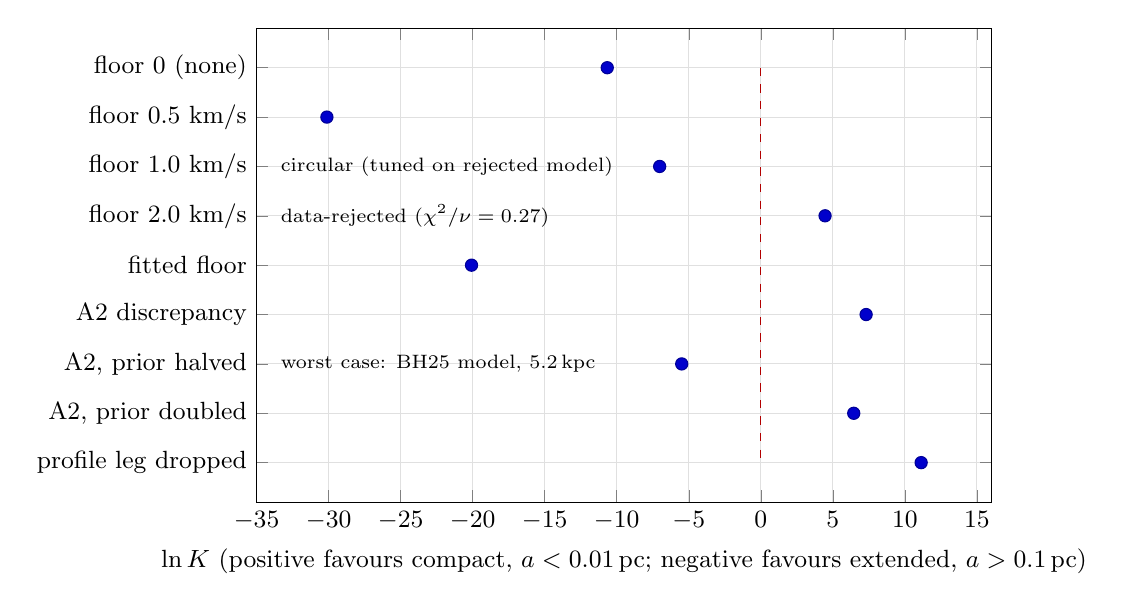
\begin{tikzpicture}
\begin{axis}[
  width=0.9\linewidth, height=7.6cm,
  xlabel={$\lnK$ (positive favours compact, $a<0.01$\,pc; negative favours extended, $a>0.1$\,pc)},
  xmin=-35, xmax=16,
  symbolic y coords={{floor 0 (none)},{floor 0.5 km/s},{floor 1.0 km/s},{floor 2.0 km/s},{fitted floor},{A2 discrepancy},{A2, prior halved},{A2, prior doubled},{profile leg dropped}},
  ytick=data, y dir=reverse,
  grid=major, grid style={black!12},
  tick label style={font=\small}, label style={font=\small},
]
\addplot+[only marks, mark=*, mark size=2.2pt, color=blue!60!black] coordinates {
  (-10.66,{floor 0 (none)})
  (-30.12,{floor 0.5 km/s})
  (-7.02,{floor 1.0 km/s})
  (4.46,{floor 2.0 km/s})
  (-20.08,{fitted floor})
  (7.31,{A2 discrepancy})
  (-5.49,{A2, prior halved})
  (6.45,{A2, prior doubled})
  (11.13,{profile leg dropped})
};
\draw[red!70!black, dashed] (axis cs:0,{floor 0 (none)}) -- (axis cs:0,{profile leg dropped});
\node[font=\scriptsize, anchor=west, align=left] at (axis cs:-34,{floor 2.0 km/s}) {data-rejected ($\chi^{2}/\nu=0.27$)};
\node[font=\scriptsize, anchor=west, align=left] at (axis cs:-34,{floor 1.0 km/s}) {circular (tuned on rejected model)};
\node[font=\scriptsize, anchor=west, align=left] at (axis cs:-34,{A2, prior halved}) {worst case: BH25 model, 5.2\,kpc};
\end{axis}
\end{tikzpicture}
\caption{The compact-versus-extended Bayes factor as a function of the profile leg's error model: each row is one labelled configuration from the amended rerun's sensitivity appendix (fiducial bracket, full prior range, Plummer visible model at 5{,}494\,pc except where labelled; the leg-dropped row spans $+10.0$ to $+12.2$ across the full bracket set, of which one configuration is plotted). The first-contact run's more extreme no-floor value ($-220$; Section~\ref{sec:fit1}) differs by normalization, not sign. Every row is an assumption choice, and the answer changes sign along the ladder. This figure is the paper's diagnosis: the profile leg does not measure the dark component's geometry; it measures the analyst's error model. The pre-registered gates (Section~\ref{sec:fit2}) formalize that reading, and the leg is retired from the verdict.}
\label{fig:ladder}
\end{figure}

\subsection{Amendment A2 and the gate battery it failed}
\label{sec:fit2}

The A2 rerun replaced every floor with the reviewed discrepancy model: a four-knot spline mean term $\delta(r)$ with Normal(0, 1.0\,\kms) knot priors, the scale fixed in advance as the quadrature budget of three named physics terms (energy-equipartition and multimass effects, 0.5--0.8\,\kms{} from the survey's own equipartition profile; flattening and azimuthal averaging at the cluster's $\epsilon \approx 0.16$; second-order rotation leakage), plus a half-Normal(0, 0.3\,\kms) white term, both marginalized everywhere, across sixteen configurations (both visible models, both distances, the primary and three mandatory companion rows). Rotation does not enter the mean model, on a mechanism ruling worth recording: the misfit lives in proper-motion dispersions computed about per-bin means, which remove ordered rotation to first order, and the measured rotation is line-of-sight in any case; the data agree, since residual rotation would inflate the tangential component and the tangential component is the low one.

All four quotability gates failed, each informatively.

\emph{The residual is component-differential.} The sign test fails in every configuration ($p = 8\times10^{-6}$ to $4\times10^{-5}$), and it fails by component: the model under-predicts the sky-radial dispersion in 33 of 40 bins and over-predicts the sky-tangential in 26 of 40, at every cell of the parameter plane, including the cell where the profile leg fits best. A shared radial discrepancy $\delta(r)$ cannot represent a component-differential residual by construction. Whatever the profile is expressing (anisotropy structure beyond one Osipkov--Merritt scale, flattening, unrelaxed substructure from the cluster's accretion origin), it is not absorbable by any radial error term, fixed or fitted.

\emph{The verdict-controlling assumption reproduces one level up.} \lnK{} fails sign unanimity (52 of 288 defined cells carry the minority sign), and the minority concentrates in the halved-prior companion row: at half the knot-prior scale, the worst configuration returns $\lnK = -5.5$ with 99\,per~cent extended posterior mass, against $+7.3$ and 97\,per~cent compact for the primary. Striking the quadrature floor moved the controlling assumption from an error-bar width to a prior width. We take the reproduction of the regress as a result, and we do not pursue a third amendment: the leg's answer is not stable under any error model we or three independent reviews could defend, because the leg does not contain the answer.

\emph{The calibration gate localizes the risk.} The injection rerun at real-data precision passes its null test with a factor-4 margin (median $|\lnK| = 0.26$ on null injections against a threshold of 1: no manufactured preference, even when the injections carry the same coherent misspecification that broke the profile leg, so the criterion-4 verdict is not an artifact of the miscalibration), recovers the correct sign in 100\,per~cent of signal injections, and covers adequately on the point-mass injection (0.86 at the primary condition), but under-covers on the extended injection: 90\,per~cent regions contain the truth 79.5\,per~cent of the time under coherent misspecification (Wilson interval 0.734--0.845, established at $n = 200$, entirely below the 0.85 requirement). The machinery is uncalibrated on the extended alternative, the one it would need most.

\emph{The kill switch fires.} The fitted discrepancy reaches 2.1--2.4\,\kms{} in the $\alpha\beta\gamma$-model configurations, beyond twice its 1.0\,\kms{} physics budget, and exceeds the budget itself in all twelve configurations. Per the pre-set fallback, the profile leg is retired from the verdict, surviving only as the visible-model calibration and as the diagnosis of this section.

Three disclosures required verbatim by Amendment A2: the discrepancy term absorbs smooth signal by construction; the profile leg's outer bins ($r > 50''$) carry no verdict-relevant signal at any systematics level compatible with the named physics; and a criterion-4 outcome under these gates is the pre-registered and publishable result.

\subsection{The fit of record, reported and not promoted}
\label{sec:record}

With the profile leg retired, the fit of record is the fast-star and pulsar joint analysis. It is stable in a way nothing else in this paper is: across both visible models, both distances, and all mass-to-light brackets, it returns $\mdark = 2.0$--$2.5\times10^{4}\,\msun$ at the point-mass limit of the grid, compact posterior mass 96--98\,per~cent, $\lnK = +10.0$ to $+12.2$ (the range over the sixteen-configuration bracket set of the amended rerun, under the reconciled mass-segregated pulsar tracer density of the released record), and a nominal, uncalibrated (per the gate of Section~\ref{sec:fit2}) 90\,per~cent upper limit of 2.2--2.7$\times10^{4}\,\msun$; its own decision-criterion tally passes in 33--34 of 36 prior cells. The optimum sits above the \citet{Haberle2024Nature} firm lower bound and a factor of a few below their model-informed range, from an analysis that shares no machinery with theirs. It also inherits the assumed Bahcall--Wolf tracer cusp inside the influence radius, a profile no dataset in this analysis measures: the mass range quoted here is conditional on that cusp, and the sensitivity to its form is a reported bracket rather than a resolved question.

We report those numbers in full and decline to quote them as a verdict, for a stated reason rather than a rhetorical one: the calibration gate failed on the extended alternative. A 96\,per~cent compact posterior from a machine that under-covers when the truth is extended is the artifact the gate exists to catch, and Amendment A2's gate clause makes the gates lexically prior to any row's tally. The pulsar accelerations contribute 3.0 nats of the joint result's dynamic range against the fast stars' 2{,}324, so the fit of record is, in substance, five stars. Five well-measured stars with a modeled selection function are genuine evidence; they are not yet a calibrated measurement, and the difference between those two sentences is this paper's method.

The pre-registered outcome therefore stands: \textbf{the data cannot decide}, criterion 4, firing on the literal pre-registration configuration and on the majority of the sixteen A2 configurations, and enforced on the remainder by the gate battery.

\section{Diagnosis: where the discriminating power actually is}
\label{sec:diagnosis}

\textbf{The dispersion profile cannot arbitrate this question at the radii that carry its weight, and there the statement is permanent at this precision.} Three independent facts compose the argument. The bins that dominate the leg's formal weight lie at $50''$--$250''$, where the dark component's enclosed-mass contribution is under $10^{-3}$: the discriminating signal is not there. The statistical errors (0.03--0.05\,\kms) sit a factor 10--40 below the leg's own physics-derived systematic budget (0.5--1.6\,\kms): the precision is not usable. And the residual against every tested model is component-differential: the systematic is not representable by any radial term. The statement is radius-resolved: it is terminal for the verdict-dominant bins beyond $\sim 50''$, while the innermost bins ($\lesssim 10''$) sit at signal-to-systematics near unity and are marginal rather than foreclosed. Deeper catalogs leave the first fact untouched and make the second worse at the verdict-dominant radii; only the inner bins can benefit, and they are a different, smaller measurement. The profile's proper role in this problem is visible-model calibration, which it performs well: the calibrated models reproduce the catalogue central escape velocity to 2--3\,per~cent without it being an input, though the catalogue value derives from models fit to overlapping kinematic data, so this is a consistency check rather than an independent one.

\textbf{The pulsar accelerations are nearly uninformative, and the analysis says so plainly.} Read correctly as censored one-sided bounds, seven usable accelerations span 3.0 nats across the entire $(\mdark, a)$ plane; alone, they bound the central mass only from above, at a prior-dominated $8.4\times10^{5}\,\msun$. The leg's real contribution is a data-quality discovery: the pre-registered posterior-predictive check on the anomalous negative accelerations discriminates between the \citet{Dai2023} and TRAPUM reductions of the same pulsars (under the Dai values, pulsar D's bound is unreachable by any model in the plane), rather than between dark-component geometries. The two reductions differ systematically in dispersion measure by 0.02--0.04\,pc\,cm$^{-3}$ across all five overlapping pulsars, far beyond either's formal errors. Until that discrepancy is resolved at the timing level, no dynamical analysis should treat either reduction's accelerations as settled input; we froze on TRAPUM as the newer, longer-baseline solution and carry Dai as the labelled sensitivity.

\textbf{The jerks are floor-limited, not precision-limited} (Section~\ref{sec:jerk}): a 1-stable nearest-neighbour floor that averaging cannot beat, discrimination requiring 5--10 times the current pulsar census, and the currently measured $\ddot{\nu}$ set inconsistent with cluster origin altogether. With the corrected $\xi$, published jerk-based significance estimates should be revisited by their authors; the correction is arithmetically small and directionally unfavorable.

\textbf{The fast stars are the live probe.} They are few, but everything about their leg behaved: stable optimum across every bracket, selection function reproducing the source paper's own contamination arithmetic, agreement with an independent analysis chain, and clean single-leg injection recovery. The two named obstacles are calibration on the extended alternative (a solvable simulation problem: the gate that failed is a coverage property of the analysis, not of the sky) and sample size (the all-seven variant fails the count posterior-predictive check in every cell, so the robust-five census is currently the informative one).

\section{The formation-physics overlay}
\label{sec:formation}

The G3 map asks, independently of all kinematics, which regions of the $(\mdark, a)$ plane published formation and retention physics can populate. Its two headline statements frame the impasse from the opposite side. The compact region implied by the fast stars ($8\times10^{3}$--$5\times10^{4}\,\msun$, $a < 0.01$\,pc) is buildable under pessimistic retention throughout: it is what the merger-growth models of \citet{GonzalezPrieto2025} produce, with recoil from the dominant, capture-driven growth channel four orders of magnitude below the escape velocity. The extended region favored by \citet{BanaresHernandez2025} is the hard one: as a pure remnant population, $2.5$--$3\times10^{5}\,\msun$ exceeds the retained black-hole mass that \citet{Dickson2024} infer for \ocen{} even at the optimistic edge of their credible range, the remainder of the region admits an all-remnant reading only at the upper edge of the published retention credible range, and every hybrid configuration that reaches the upper masses requires an embedded IMBH of $1.5$--$6.6\times10^{4}\,\msun$, which the extended solution's own $3\sigma$ point-mass cap excludes. The upper half of the extended region is reachable, on published physics, only through configurations the extended fit itself rules out.

Formation physics and the profile-driven kinematics thus point in opposite directions, and the overlay is carried as exactly that: a live disagreement, reported alongside the posterior, tilting nothing (the map never enters the likelihood). A dynamical caution cuts the same way: an extended $3.5\times10^{4}\,\msun$ remnant configuration at $0.2$\,pc scale, the kind of solution the unrepaired profile leg preferred, has a subsystem relaxation time of order $10^{5}$\,yr and does not persist; where the misfitting fit parked its posterior was not a physical configuration at all.

\section{What would decide it}
\label{sec:decide}

In order of leverage per unit effort. \textbf{(i) Calibrate the fast-star machinery on the extended alternative.} The failed gate is a simulation deliverable: extended-truth injection campaigns at real precision until coverage is demonstrated, then the fit of record's verdict becomes quotable at whatever strength survives. No new data required. \textbf{(ii) Resolve the Dai/TRAPUM timing discrepancy.} A timing-level reconciliation of the DM offsets and of pulsar B's derivative sign, by the groups that own the data; until then every acceleration-based claim about this cluster inherits it. \textbf{(iii) Enlarge the fast-star census.} The robust five carry the result; the existing astrometric archive plus one more epoch of the same quality would either populate the tail or bound it. \textbf{(iv) An anisotropy-structured profile analysis.} The component-differential residual is a named, measured target (radial under-predicted, tangential over-predicted, at every radius); a separately pre-registered campaign with component-resolved discrepancy modeling, or axisymmetric machinery, addresses what this paper's shared radial term could not. It would improve the visible model and could open the marginal inner bins; on the terminality argument above, the verdict-dominant outer profile should not be expected to arbitrate under any version of it. \textbf{(v) More timed pulsars.} At a census of order $10^{2}$, jerks activate as a genuinely independent channel \citep{Abbate2019,ChenPTA2025}; the corrected floor makes the requirement concrete, with the finalized forecast flagged for the released record.

\section{Conclusion}
\label{sec:conclusion}

We pre-registered a joint analysis of the contested central dark mass of \ocen, validated it adversarially, ran it, amended its error model once under independent review, and report the pre-registered null: the data cannot yet decide between a compact and an extended central dark mass. The analysis localizes the indecision. The dispersion profile, the formally strongest dataset, cannot arbitrate the question at any error model, because its precision lies at radii that carry no discriminating signal and its residual structure is not radial; the pulsar accelerations are censored into near-silence; the jerks sit under a 1-stable floor that no timing precision escapes, with a corrected constant that other groups can verify in one line of algebra. What remains live is small and specific: five robust fast stars whose stable compact preference awaits a demonstrated calibration, a formation-physics overlay that builds the compact solution easily and the extended one only through self-excluded hybrids, and a short, ordered list of what would settle it. The mass tension of \ocen{} is not a disagreement between datasets; it is a disagreement between assumptions that the datasets are not yet strong enough to overrule --- and now there is a measurement of exactly how strong they would need to be.

\section*{Data availability}
The complete analysis chain is distributed with the paper source at omegacentauri.me: the pre-registration with its full git history and both amendments; the provenance-annotated data extractions with content hashes; the validation reports for gates G1--G3 with fixed seeds; both fit reports with every configuration, gate verdict, and sensitivity row; the three independent methodological reviews behind Amendment A2; and a self-audit script that re-derives every number quoted in the fit reports from the released result files (140 checks); superseded result blocks are marked in situ in the released files. The provenance chain includes its own error record: a factor-of-ten transcription slip in an early digitized anisotropy anchor was caught by the subsequent checksum-verified file retrieval and is documented, with both values, in the released extraction, which is the discipline this paper's conclusions depend on working in practice.

\section*{Acknowledgements}
This analysis rests on the public data products of the oMEGACat survey, the TRAPUM collaboration, and the SDSS-V Local Volume Mapper, and on the published formalisms of Prager et al. and Abbate et al., whose jerk framework we correct in one constant and otherwise reproduce with admiration.

\bibliographystyle{apalike}
\bibliography{references,masstension-extra}

\end{document}
